\documentclass[a4paper,12pt]{article}

%%% Работа с русским языком
\usepackage{cmap}					% поиск в PDF
\usepackage{mathtext} 				% русские буквы в фомулах
\usepackage[T2A]{fontenc}			% кодировка
\usepackage[utf8]{inputenc}			% кодировка исходного текста
\usepackage[english,russian]{babel}	% локализация и переносы

%%% Дополнительная работа с математикой
\usepackage{amsfonts,amssymb,amsthm,mathtools} % AMS
\usepackage{amsmath}
\usepackage{icomma} % "Умная" запятая: $0,2$ --- число, $0, 2$ --- перечисление

%% Номера формул
%\mathtoolsset{showonlyrefs=true} % Показывать номера только у тех формул, на которые есть \eqref{} в тексте.

\usepackage{hyperref}
\hypersetup{
    colorlinks=true,
    linkcolor=blue,
    filecolor=magenta,      
    urlcolor=cyan,
}

\usepackage{float}


%% Шрифты
\usepackage{euscript}	 % Шрифт Евклид
\usepackage{mathrsfs} % Красивый матшрифт

%%% Работа с картинками
\usepackage{graphicx}  % Для вставки рисунков
\graphicspath{{images/}{images2/}}  % папки с картинками
\setlength\fboxsep{3pt} % Отступ рамки \fbox{} от рисунка
\setlength\fboxrule{1pt} % Толщина линий рамки \fbox{}
\usepackage{wrapfig} % Обтекание рисунков и таблиц текстом
\usepackage{caption}
\usepackage{subcaption}
\captionsetup{labelsep=period} %. вместо : в рис

\title{Научный отчёт по проекту Решеточные модели макромолекул}
\author{Москаленко Роман}
\date{}

\begin{document}

\maketitle

\section{Цель проекта}

Разработка программного комплекса моделирования модели Изинга на ансамблях случайных графов  для последующего исследования их термодинамических характеристик.


\section{Алгоритмы}

Реализованы два алгоритма обновления спинов. Односпиновый и кластерный апдейт. Оба алгоритма работают на произвольном графе, используя таблицу соседей. Алгоритмы реализованы как отдельные библиотеки для Python, и написаны с использованием технологии Cython для ускорения работы. Кластерный апдейт является более эффективным по времени работы и количеству шагов, которые необходимо выполнить для хорошей сходимости модели.

\subsection{Проверка алгоритмов}

Чтобы убедиться что алгоритмы работают правильно мы проверили, что оба алгоритма дают одинаковые результаты на одних и тех же конформациях, так же сравнил их с точными решениями для одномерной модели Изинга.

Результаты замеров кластерным и односпиновым апдейтом совпадают в пределах погрешности.

\begin{figure}[H]
	\centering
	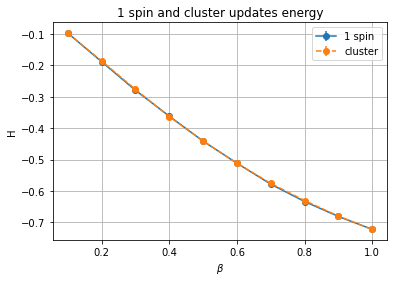
\includegraphics[width = 0.45\textwidth]{../images/1spin_&_cluster_ene.png} 
	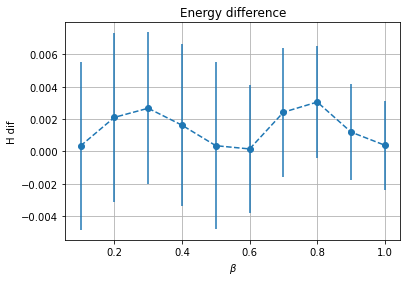
\includegraphics[width = 0.45\textwidth]{../images/1spin_&_cluster_ene_dif.png} 
	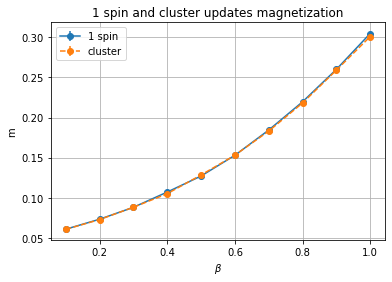
\includegraphics[width = 0.45\textwidth]{../images/1spin_&_cluster_mag.png} 
	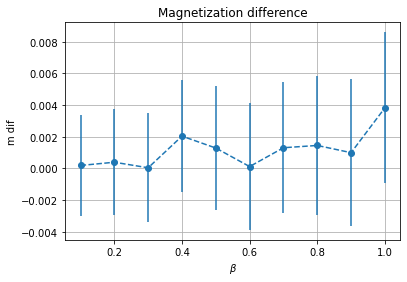
\includegraphics[width = 0.45\textwidth]{../images/1spin_&_cluster_mag_dif.png} 
	%% add magnetization
	\caption{кластерный и односпиновый апдейт}
\end{figure}

Для сравнения с точными значениями для одномерной модели Изинга, мы используем замкнутый квадратный контур. Данная конформация по свойствам полностью совпадает с одномерной моделью Изинга с открытыми граничными условиями.

\begin{figure}[H]
	\centering
	\begin{subfigure}[t]{0.45\textwidth}
		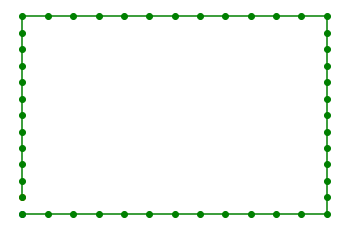
\includegraphics[width = \textwidth]{../images/1D_conf.png} 
		\caption{Конформация эмитирующая одномерную модель}
	\end{subfigure}
	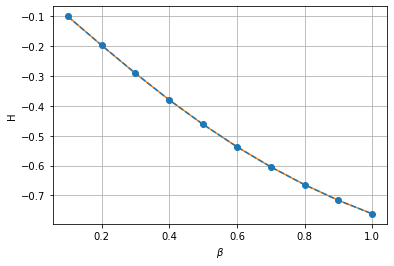
\includegraphics[width = 0.45\textwidth]{../images/1D_ene.png}
	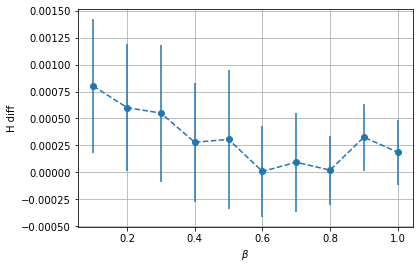
\includegraphics[width = 0.45\textwidth]{../images/1D_ene_diff.png} 
	%% add magnetization
	\caption{Сравнение с точным решением одномерной модели}
\end{figure}

Так же был написан код, точно вычисляющий энергию системы путём полного перебора всех её состояний. Сравнение на маленьких конформациях (длина 10) даёт одинаковые результаты.

%TODO втавить результаты поного перебора

Примеры с использованием кластерного апдейта добавлены в библиотеку \texttt{mc\_lib}.

\section{Текущие результаты замеров}
Пока что замеры проводилиь только для конформаций сгенерированных в двумерном пространстве.
 
Как и ожидалось, неплотыне конформации оказались близки к одномерной модели изинга, в них не возникает намагниченность и нет фазового перехода. В свою очередь плотные графы близки к двумерной модели, и намагничиваются при низких температурах.

\begin{figure}[h]
	\centering
	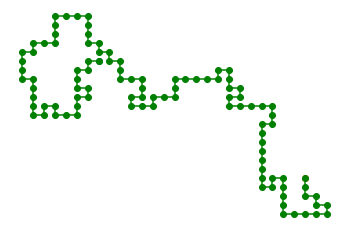
\includegraphics[width=0.45\textwidth]{../images/loose_conf.png}
	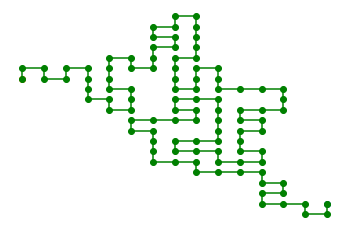
\includegraphics[width=0.45\textwidth]{../images/dense_conf.png} 
	%% add magnetization
	\caption{Пример неплотной и плотной конформации}
\end{figure}

В данный момент я занимаюсь нахождением точки фазового перехода в плотных графах.



\end{document}